\documentclass[UTF8]{ctexart}
\usepackage{subfigure}
\usepackage{caption}
\usepackage{amsmath,bm}
\usepackage{amssymb}
\usepackage{pifont}
\usepackage{geometry}
\usepackage{graphicx}
\usepackage{gensymb}
\usepackage{wrapfig}
\usepackage{titlesec}
\usepackage{float}
\usepackage{diagbox}
\usepackage{fancyhdr}
\usepackage{color}
\usepackage{bm}
\pagestyle{plain}
\geometry{a4paper,scale=0.8}
\CTEXsetup[format+={\raggedright}]{section} 
\title{固物2019期中(A卷)}
\author{Deschain}
\titlespacing*{\section}
{0pt}{0pt}{0pt}
\titlespacing*{\subsection}
{0pt}{0pt}{0pt}
\titlespacing*{\paragraph}
{0pt}{0pt}{0pt}
\titlespacing*{\subparagraph}
{0pt}{0pt}{0pt}
\titleformat*{\section}{\normalsize}
\begin{document}
\maketitle
\section*{\bfseries 1.填空题(每题1分,共40分)}
(1)设金属中价电子(自由电子)密度为$n$,电子质量为$m$,则$0K$时费米球半径为\uline{\makebox[6em]{}},
费米能量为\uline{\makebox[8em]{}}。温度高于绝对零度时,费米能量\uline{\makebox[4em]{}}(略低、等
于、略高)于绝对零度时的费米能量。\\
(2)室温下,金属材料的费米能级位于\uline{\makebox[4em]{}}(导带、价带、禁带)中。绝对零度条件下,金属导
带中电子填充情况为\uline{\makebox[6em]{}},半导体导带中电子填充情况为\uline{\makebox[6em]{}}。\\
(3)若电子占据了一个能带中所有的状态,则该能带\uline{\makebox[3em]{}}(能/不能)导电;没有电子的能带
\uline{\makebox[3em]{}}(能/不能)导电。\\
(4)布拉菲点阵中,能够完全平移覆盖的最小单元称为\uline{\makebox[3em]{}}。\\
(5)晶体中的缺陷按其几何特征可以分为\uline{\makebox[2em]{}}缺陷、\uline{\makebox[2em]{}}缺陷和
\uline{\makebox[2em]{}}缺陷。其中位错是一种典型的\uline{\makebox[2em]{}}缺陷,可以分为
\uline{\makebox[3em]{}}位错和\uline{\makebox[3em]{}}位错。\\
(6)Cu、Au、Ag、Al等金属的晶格属于\uline{\makebox[6em]{}}晶格,其原子排列最致密的等效晶面的密勒指数是
\uline{\makebox[4em]{}}。\\
(7)假设$GaAs$晶体的晶格常数为$a$,则最近邻$Ga$和$As$原子的间距为\uline{\makebox[3em]{}};两个最近邻
$As$原子的间距为\uline{\makebox[6em]{}}。\\
(8)金刚石中$C-C$键结合的方式是典型的\uline{\makebox[6em]{}};除了这种结合方式外,固体的结合方式还有
\uline{\makebox[6em]{}}、\uline{\makebox[6em]{}}、\uline{\makebox[9em]{}}。\\
(9)元素周期表中,越往上或越往右,元素的负电性\uline{\makebox[3em]{}}(填越小或越大),说明原子在形成化
学键时对成键电子的吸引力\uline{\makebox[3em]{}}(填越小或越大)。\\
(10)$Si$的晶体结构是\uline{\makebox[4em]{}},其布拉菲格子是\uline{\makebox[6em]{}}格子,与之对应
的倒格子则是\uline{\makebox[6em]{}}格子。假设$Si$的晶格常数为$a$,则其布拉菲格子原胞的体积为
\uline{\makebox[3em]{}},而其倒格子的晶格常数为\uline{\makebox[3em]{}},第一布里渊区的体积为
\uline{\makebox[3em]{}}\\
(11)一般用$X$射线衍射实验来研究晶体的微观结构,这是由于\uline{\makebox[7em]{}}与晶格常数相当,能够发生晶
体衍射现象。\\
(12)在能带理论中,将周期性势场看做弱晶格近似势近似求解薛定谔方程的方法称为\uline{\makebox[10em]{}},在该
条件下,可以使用\uline{\makebox[3em]{}}理论来逐级求解电子波函数和能量本征值。其中,零极哈密顿量与\\
\uline{\makebox[12em]{}}中的一致。\\
(13)自由电子的$E-k$关系图为\uline{\makebox[3em]{}}线型,但是在晶格的周期势场中,电子的能量会在$k$的取值为
\uline{\makebox[19em]{}}时产生劈裂,从而在$E-k$关系图中出现\uline{\makebox[3em]{}}。\\
(14)晶体中原子排列的空间频率用\uline{\makebox[4em]{}}来表述。在晶体衍射实验中,得到的衍射图样实际上就是晶
体的\uline{\makebox[4em]{}}的映像。\\
\section*{\bfseries 2.简答题(每题5分,共20分)}
(1)波矢空间与倒格空间有什么联系?这两个空间中的格点分布有什么区别?\\
(2)请简述原胞、单胞(惯用原胞)的的区别。\\
(3)请简述在晶体结合中结合能的概念,结合能与内能的关系以及结合能与原子间相互作用力的关系。\\
(4)请利用近自由电子模型简述晶体中电子的带隙产生的原因。为什么不同的晶体其带隙大小不同?\\
\section*{\bfseries 3. 原图缺失}
\section*{\bfseries 4.(10分)如将晶格常数为$a$的立方晶系布拉菲格子的格矢量$R$在互相正交的单位矢量
$\bm{i},\bm{j},\bm{k}$组成的直角坐标系中表示为$R=\frac{a}{2}(n_1\bm{i}+n_2\bm{j}+n_3\bm{k})$,其中$n_1,n_2$
和$n_3$为整数。 求:}
(1)若为体心立方格子,系数$n_1,n_2$和$n_3$需要满足什么条件?\\
(2)若为面心立方格子,系数$n_1,n_2$和$n_3$需要满足什么条件?\\
\section*{\bfseries 5.(8分)电子在一维周期势场中运动,晶格常数为$a$}
(1)周期势场的表达式为$V(x)=2+cos(\frac{2\pi}{a}x)cos(\frac{4\pi}{a}x)
+\frac{1}{2}sin(\frac{2\pi}{a}x)sin(\frac{6\pi}{a}x)$,请求出$V(x)$的各级傅里叶展开系数。\\
(2)在简约布里渊区图景中画出对应于该周期势场的电子的$E-k$关系示意图,并标注带隙大小。\\
\section*{\bfseries 6.原图缺失}
\section*{\bfseries 7.$U(r)=4\varepsilon[(\frac{\sigma}{r})^{12}-(\frac{\sigma}{r})^6]$,其中$\varepsilon,\sigma$
为雷纳德-琼斯参数,它们均大于0且分别与$U,r$具有相同量纲。}
(1)求出该惰性气体原子的平衡间距。\\
(2)说明雷纳德-琼斯参数$\varepsilon,\sigma$的物理意义。\\



\newpage
\section*{\bfseries 1.填空题答案}
(1)\ding{172}$(3\pi^2 n)^{\frac{1}{3}}$ \makebox[2em]{} 
\ding{173}$\frac{\hbar^2}{2m}(3\pi^2 n)^{\frac{2}{3}}$\makebox[2em]{}  
\ding{174}略低\\
(2)\ding{172}导带\makebox[2em]{}  
\ding{173}部分填充\makebox[2em]{}
\ding{174}空带(没有电子填充)\\
(3)\ding{172}不能\makebox[2em]{}
\ding{173}不能\\
(4)\ding{172}原胞\\
(5)\ding{172}点\makebox[2em]{}
\ding{173}线\makebox[2em]{}
\ding{174}面\makebox[2em]{}
\ding{175}线\makebox[2em]{}
\ding{176}刃形\makebox[2em]{}
\ding{177}螺形\\
(6)\ding{172}面心立方\makebox[2em]{}
\ding{173}$\{111\}$\\
(7)\ding{172}$\frac{\sqrt2}{4}a$\makebox[2em]{}
\ding{173}$\frac{\sqrt2}{2}a$\\
(8)\ding{172}共价结合\makebox[2em]{}
\ding{173}离子结合\makebox[2em]{}
\ding{174}金属性结合\makebox[2em]{}
\ding{175}范德瓦尔斯结合\\
(9)\ding{172}越大\makebox[2em]{}
\ding{173}越大\\
(10)\ding{172}金刚石\makebox[2em]{}
\ding{173}面心立方\makebox[2em]{}
\ding{174}体心立方\makebox[2em]{}
\ding{175}$\frac{a^3}{4}$\makebox[2em]{}
\ding{176}$\frac{4\pi}{a}$\makebox[2em]{}
\ding{177}$32(\frac{\pi}{a})^3$\\
(11)$X$射线波长\\
(12)\ding{172}近自由电子近似\makebox[2em]{}
\ding{173}微扰\makebox[2em]{}
\ding{174}索末菲自由电子近似\\
(13)\ding{172}抛物\makebox[2em]{}
\ding{173}布里渊区边界\makebox[2em]{}
\ding{174}带隙\\
(14)\ding{172}倒格矢\makebox[2em]{}
\ding{173}倒格子\\
\section*{\bfseries 2.简答题答案}
(1)\ding{172}波矢空间和倒格空间处于同一空间。\\
\ding{173}倒格空间的基矢分别为$\bm{b_1},\bm{b_2},\bm{b_3}$,
而波矢空间的基矢分别为$\frac{\vec{b_1}}{N_1},\frac{bm{b_2}}{N_2},\frac{\bm{b_3}}{N_3}$,
$N_1,N_2,N_3$分别为沿正格子基矢方向晶体的原胞数目。波矢空间每个格点占有的体积是倒格空间每个格点体积的
$\frac{1}{N}$,$N=N_1\times N_2\times N_3$。简而言之,波矢空间比倒格空间格点排列更密。\\
(2)\ding{172}原胞是体积最小的晶胞,只含有一个格点,是可以完全平移覆盖点阵结构的最小单元,原胞的边矢量称为晶格基矢。\\
\ding{173}单胞可以包含多个格点,是点阵中可以完全平移覆盖、并能体现旋转对称性的常用单元。单胞的边矢量长度为晶格常数。\\
(3)\ding{172}分散的自由原子结合成为晶体的过程中释放出来的能量称为结合能。\\
\ding{173}以无穷远处分散的原子状态为能量零点,定义晶体结合后稳定时内能最小值$U(r_0)=-W$即结合能为$W=-U(r_0)$。\\
\ding{174}$r=r_0$时,原子间相互作用力为从吸引力转为排斥力的拐点。\\
(4)\ding{172}在近自由电子近似模型中,晶格的周期性势场被看做微扰。在布里渊区的边界,波函数是简并的。根据简并微扰模型,会发生能级
劈裂,也就形成了带隙。\\
\ding{173}不同晶体原子的空间排列方式不同,形成的周期性势场也是不同的,所以带隙大小是不同的。\\
\section*{4.解答}
布拉菲格子的晶格平移矢量可表示为
\begin{equation}
    \begin{aligned}
        & R_{lmn}=l\bm{a_1}+m\bm{a_2}+n\bm{a_3}\\
    \end{aligned}
\end{equation}
的形式,其中$\bm{a_1},\bm{a_2},\bm{a_3}$是布拉菲格子的基矢,$l,m,n$是整数。\\
(1)将体心立方格子的基矢$\bm{a_1}=\frac{a}{2}(-\bm{i}+\bm{j}+\bm{k}),\bm{a_2}=\frac{a}{2}(\bm{i}-\bm{j}+\bm{k}),
\bm{a_3}=\frac{a}{2}(\bm{i}+\bm{j}-\bm{k})$代入式(1)中,得
\begin{equation*}
    \begin{aligned}
        & R_{lmn}=\frac{a}{2}[(-l+m+n)\bm{i}+(l-m+n)\bm{j}+(l+m-n)\bm{k}]=\frac{a}{2}(n_1\bm{i}+n_2\bm{j}+n_3\bm{k})\\
    \end{aligned}
\end{equation*}
由于$l,m,n$都是整数,$n_1,n_2,n_3$之间两两的差值为偶数,因此$n_1,n_2,n_3$只能全部是奇数或偶数。\\
(2)类似地,面心立方格子的晶格平移矢量可表示为
\begin{equation*}
    \begin{aligned}
        & R_{lmn}=\frac{a}{2}[(m+n)\bm{i}+(l+n)\bm{j}+(l+m)\bm{k}]=\frac{a}{2}(n_1\bm{i}+n_2\bm{j}+n_3\bm{k})\\
    \end{aligned}
\end{equation*}
则
\begin{equation*}
    \begin{aligned}
        & n_1=m+n,n_2=n+l,n_3=l+m
    \end{aligned}
\end{equation*}
因此$n_1+n_2+n_3=2(l+m+n)$的和为偶数。\\
\section*{5.解答}
(1)
\begin{equation*}
    \begin{aligned}
        & V(x)=2+\frac{1}{4}e^{i\frac{2\pi}{a}x}+\frac{1}{4}e^{-i\frac{2\pi}{a}x}-\frac{1}{8}e^{i\frac{4\pi}{a}x}
        -\frac{1}{8}e^{-i\frac{4\pi}{a}x}+\frac{1}{4}e^{i\frac{6\pi}{a}x}+\frac{1}{4}e^{-i\frac{2\pi}{a}x}
        +\frac{1}{8}e^{i\frac{8\pi}{a}x}+\frac{1}{8}e^{-i\frac{8\pi}{a}x}\\
        & V_0 = 2, V_{\pm1}=\frac{1}{4}, V_{\pm2}=-\frac{1}{8}, V_{\pm3}=\frac{1}{4}, V_{\pm4}=\frac{1}{8}
    \end{aligned}
\end{equation*}
(2)
\begin{figure}[H]
    \centering
    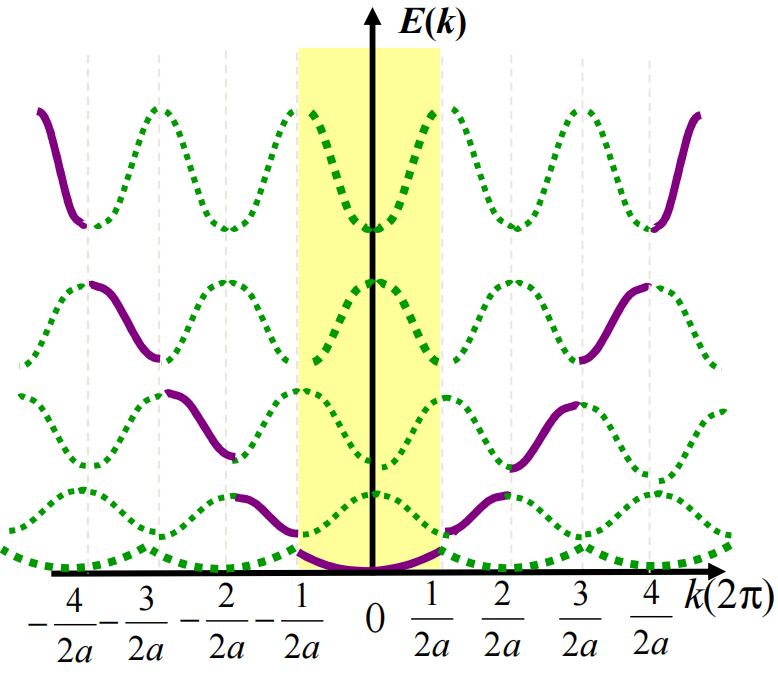
\includegraphics[width=4cm,height=4cm]{5.png}
\end{figure}
\section*{\bfseries 7.解答}
(1)设平衡间距为$r_0$
\begin{equation*}
    \begin{aligned}
        & \frac{dU(r)}{dr}=24\varepsilon\sigma^6(-\frac{2\sigma^6}{r^{13}}+\frac{1}{r^7})\\
        & \frac{dU(r_0)}{dr}=0, r_0=2^{\frac{1}{6}}\sigma\\
    \end{aligned}
\end{equation*}
(2)$U(r_0)=-\varepsilon,\varepsilon$是原子的结合能。\\
$U(\sigma)=0,\sigma$是相互作用能为0时的原子间距。\\












\end{document}